\chapter{Design Model: Distributed Managed Systems (DREMS)}
\label{chapter:DREMS}

\section{DREMS Component Model}

Timing analysis of component-based software is facilitated by the the DREMS infrastructure (\iapfull) \cite{DREMS13Software}, \cite{ISIS_F6_ISORC:13}. DREMS was designed and implemented for a class of distributed real-time embedded systems that are remotely deployed and are characterized by strict timing requirements e.g. a cluster of satellites. DREMS is a software infrastructure for the design, implementation, deployment and management of component-based real-time embedded systems. The infrastructure includes design-time modeling tools \cite{ISIS_F6_SFFMT:13} that integrate with a well-defined and fully implemented component model \cite{ISIS_F6_ISORC:13, kumar2014colored} used to build component-based applications. Rapid prototyping and code generation features coupled with a modular runtime platform automate the tedious aspects of the software development and enable robust deployment and operation of mixed-criticality distributed applications.

The DREMS component model is based on the Component Integrated ACE ORB (CIAO) \cite{RT_CIAO:04, CIAO_Chap:04} project. CIAO is an implementation of the OMG's Lightweight CORBA Component Model (CCM) \cite{CCM-light:03}. CIAO uses the
TAO~\cite{TAO:02} CORBA object request broker (ORB) as its default underlying
communication middleware.  With the recent standardization of connector mechanisms~\cite{dds4ccm:09}, CIAO is also able to support asynchronous messaging and the OMG Data Distribution Service (DDS) through its ports. Unlike CIAO, the DREMS component model is not tightly coupled with the CORBA transport mechanisms. All component communication is via ports and connectors \cite{Connectors} enabling a variety of interaction schemes. For safe and deadlock-free behavior, this component model also allows only one thread of control per component to be active at any given instant of time. 

\begin{figure}[h]
	\centering
	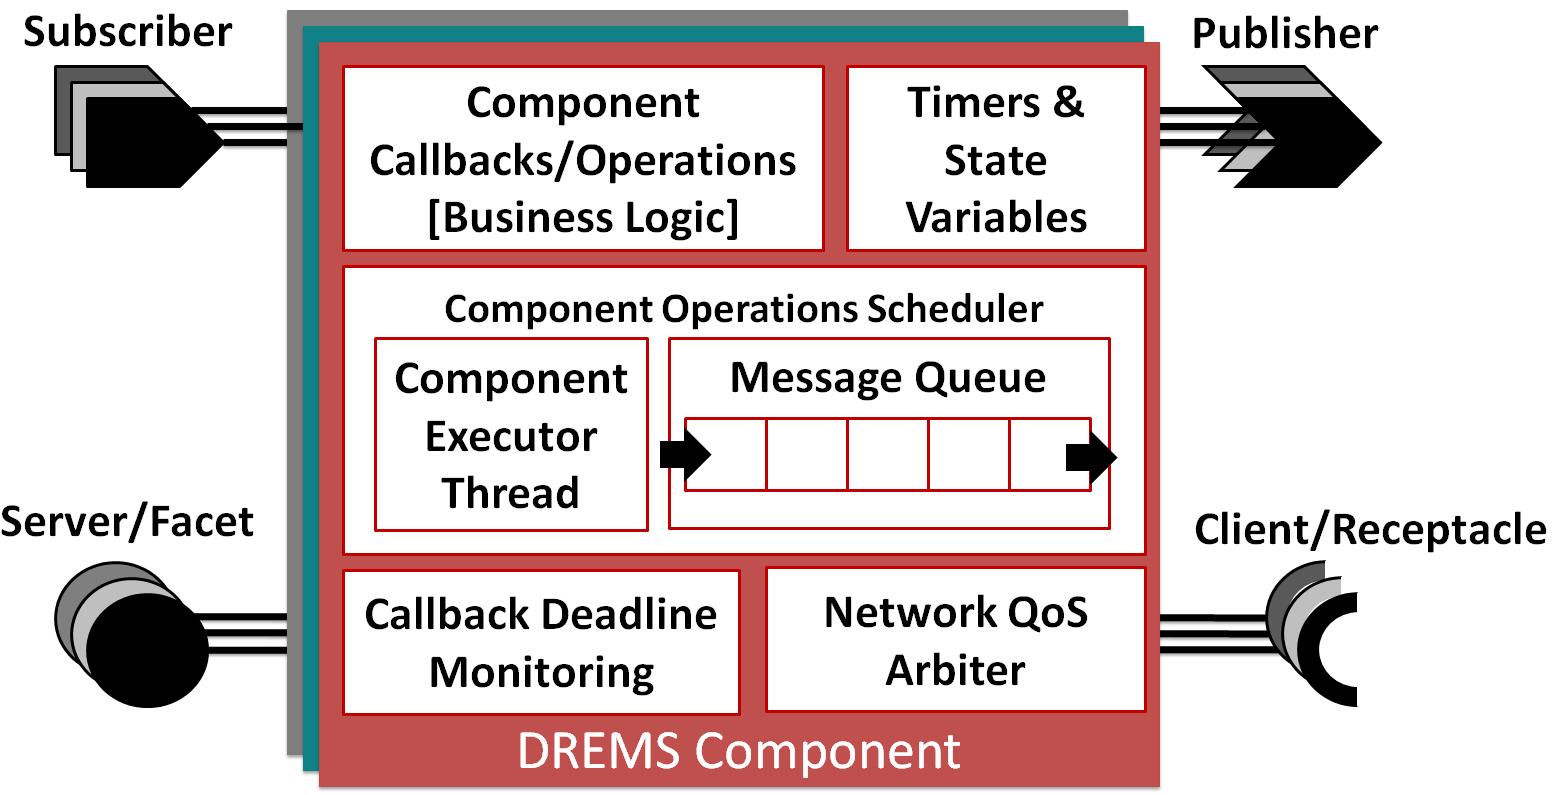
\includegraphics[width=\textwidth]{DREMS_Component}
	\caption{DREMS Component}
	\label{fig:DREMS_Component}
	\vspace{-0.1in}
\end{figure}


Figure \ref{fig:DREMS_Component} presents a typical DREMS-style component. Component-based software engineering relies on the principle of assembly: Large and complicated systems can be iteratively constructed by composing small reusable component building blocks. Each \emph{component} contains a set of communication ports and interfaces, a message queue, time-triggered event handling and state variables. Using ports, components communicate with the external world. Using interfaces and message passing schemes, components process requests from other components. This interaction mechanism lies at the heart of component-based software. 

Each DREMS component supports four basic types of ports for interaction with other collaborating components: Facets, Receptacles, Publishers and Subscribers. A component's {\bf facet} is a unique interface that it exposes to its clients. This interface can be invoked either synchronously via remote method invocation (RMI) or asynchronously via asynchronous method invocation (AMI) \cite{waldo1998remote, raje1997asynchronous}. A component's {\bf receptacle} specifies an interface required by the component in order to function correctly. Using its receptacle, a component can establish connections and invoke operations on other components using either RMI or AMI. A {\bf publisher} port is a single point of data emission. This port emits data produced by a component operation. A {\bf subscriber} port is a single point of data consumption, feeding received data to the associated component. Communication between publishers and subscribers is contingent on the compatibility of their associated topics. Publishers and Subscribers enable the OMG DDS anonymous publish/subscribe \cite{eugster2003many} style of messaging. More details on this component model can be found in ~\cite{ISIS_F6_ISORC:13}.

\section{Component Operations}

An \emph{operation} is an abstraction for the different tasks undertaken by a component. These tasks are implemented by the component's executor code written by the developer. Application developers provide the functional, \emph{business-logic} code that implements operations on the state variables e.g. a PID control operation could receive the current state of dynamic variables from a \emph{Sensor} Component, and using the relevant gains, calculate a new state to which an \emph{Actuator} component should progress the system. In order to service interactions with the underlying framework and with other components, every component is associated with a \emph{message queue}. This queue holds instances of operations ('messages') that are ready for execution and need to be serviced by the component. These operations service either interaction requests (seen on communication ports) or service requests (from the underlying framework). An example for the latter is the use of component timers that can periodically (or sporadically) activate an operation. 

Figure \ref{fig:component_operations} shows this model. Each operation is characterized by a priority and a deadline. Operation deadlines are quantified in absolute time measured starting from when the operation is enqueued onto the component message queue. These operations are sorted and scheduled based on one of three scheduling schemes: Earliest Deadline First (EDF), First In First Out (FIFO), or Priority FIFO (PFIFO). 

\begin{figure}[ht]
	\centering
	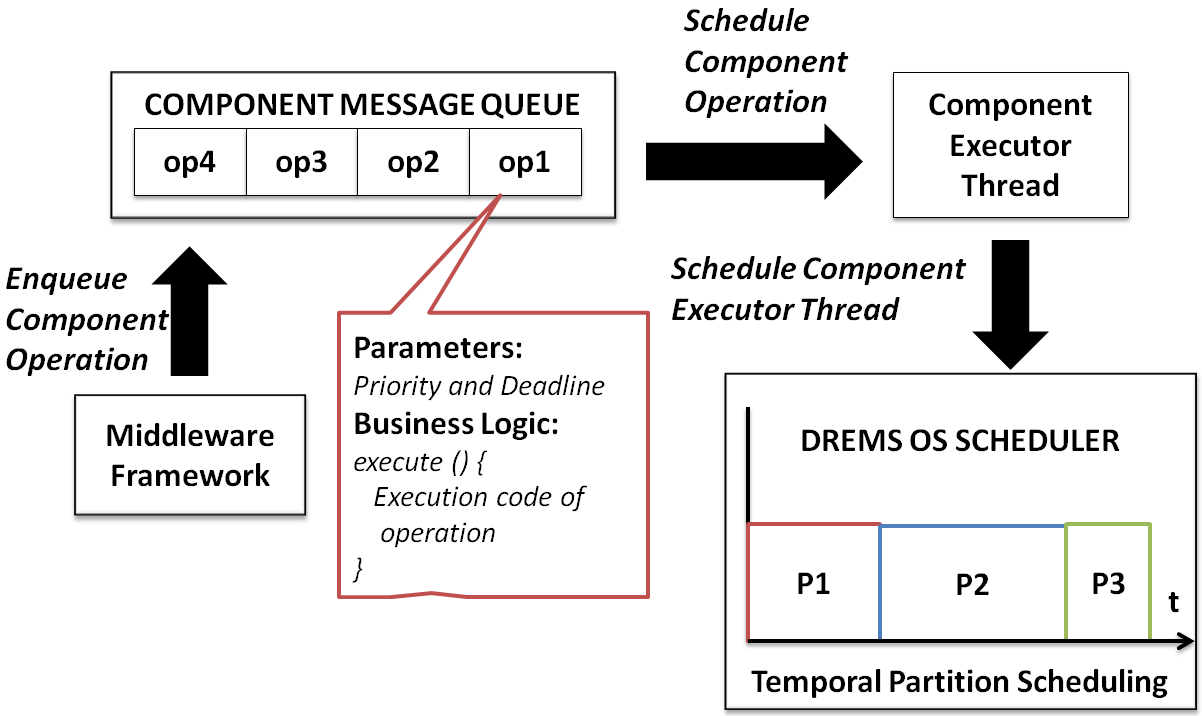
\includegraphics[width=\textwidth]{component_operations}
	\caption{Scheduling Component Operations}
	\label{fig:component_operations}
\end{figure}
%\vspace{0.2in}

To facilitate component behavior that is free of deadlocks and race conditions, the component's execution is handled by a single thread. Operations in the message queue are therefore scheduled one at a time under a non-preemptive policy. A component dispatcher thread dequeues the next ready operation from the component message queue. This operation is scheduled for execution on a component executor thread. The operation is run to completion before another operation from the queue is serviced. This single-threaded execution helps avoid synchronization primitives such as internal state variables that lead to strenuous code development. Though components that share a processor still run concurrently, each component operation is executed by a single component-specific executor thread.

\begin{figure}[ht]
	\centering
	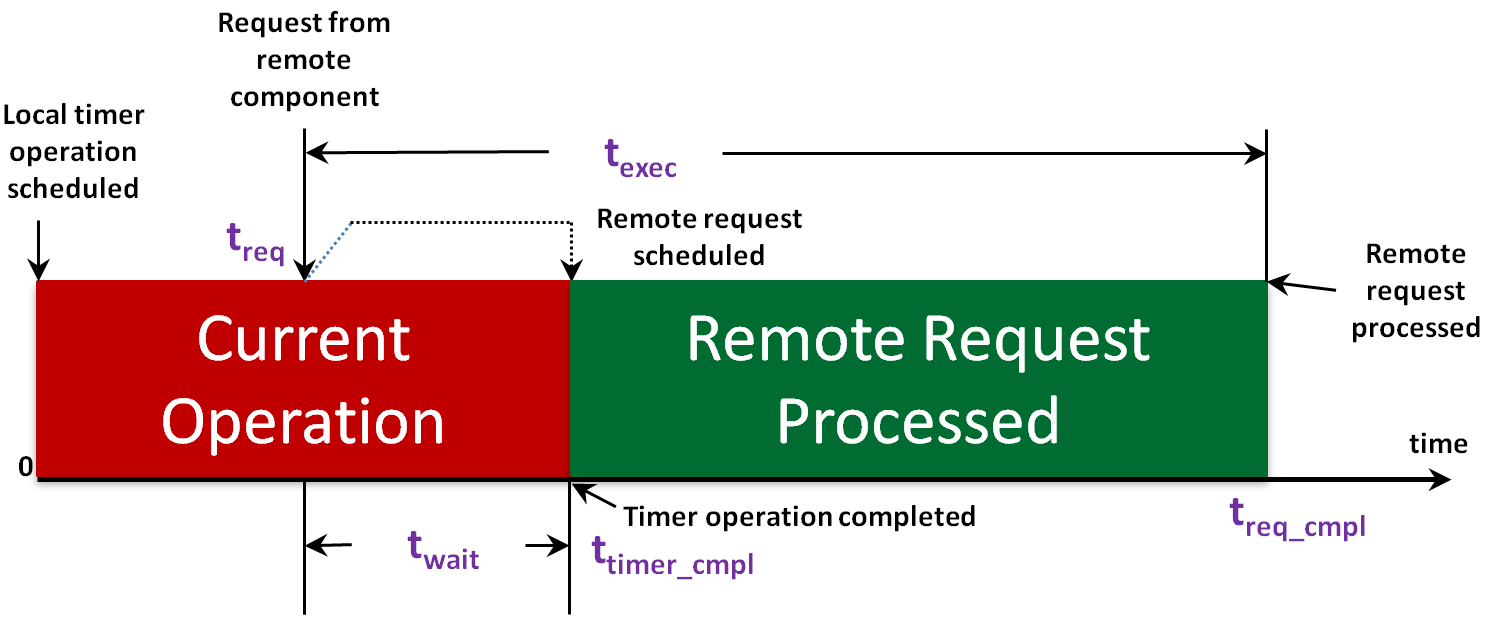
\includegraphics[width=\textwidth]{cop_execution_semantics}
	\caption{Component Operation - Execution Semantics}
	\label{fig:cop_execution_semantics}
\end{figure}

Figure \ref{fig:cop_execution_semantics} shows the execution semantics of a component operation executed on a lone component executor thread. A simplifying assumption  to describe the semantics is that this component is the only component thread executing on this CPU. Assume that at $t=0$, this component is processing the expiry of a local timer. This operation is expected to complete at $t = t_{timer\_cmpl}$. However, at $t = t_{req}$, a service request is received from some remote component. Since the component operation scheduling is non-preemptive, regardless of the priority of this service, the request is not processed until $t_{next}$. Therefore, the request is waiting in the message queue for $t_{wait} = t_{timer\_cmpl} - t_{req}$. At $t = t_{timer\_cmpl}$, the timer operation is marked as complete and the service request is processed. The total execution time of this service operation is calculated including the duration of the time for which this request waited in the component message queue i.e. $t_{exec} = t_{req\_cmpl} - t_{req}$. The wait times in the queue are further worsened when OS scheduling non-determinism is taken into account. There are specifically three ways in which the OS scheduling can delay operations: (1) if the application process is concurrently executing multiple component threads, then the threads are scheduled in Round-Robin fashion by the OS, (2) when mixed-criticality application processes are scheduled in tandem, the OS uses fixed-priority Round-Robin scheduling to schedule the process threads, and finally (3) temporally partitioned OS schedules further cause delays on component thread scheduling, which directly affects the scheduling and timely completion of component operations. 

\section{Temporal Partition Scheduler}

DREMS components are grouped into processes that are assigned to temporal partitions, implemented by the DREMS OS scheduler. This scheduler was implemented by modifying the behavior of the standard Linux scheduler, introducing an ARINC-653 ~\cite{ARINC-653} style temporal and spatial partitioning scheme. 

\begin{figure}[ht]
	\centering
	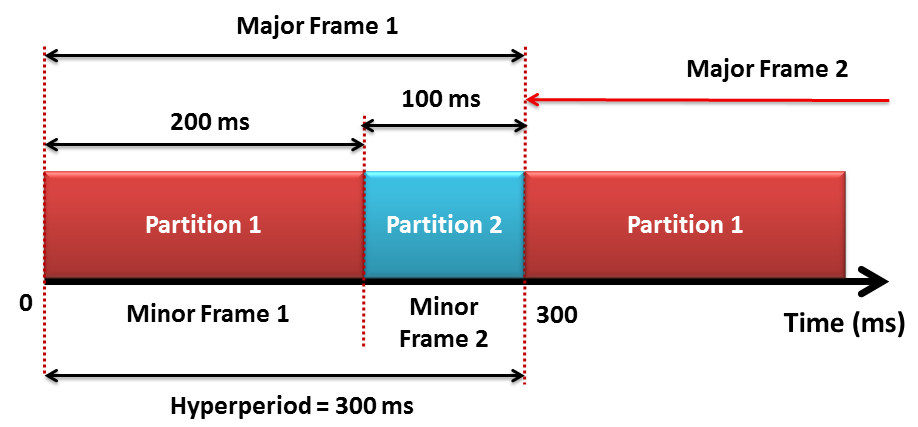
\includegraphics[width=\textwidth]{partition_scheduling}
	\caption{Sample Temporal Partition Schedule with Hyperperiod = 300 ms}
	\label{fig:partition_scheduling}
\end{figure}


Temporal partitions are periodic fixed intervals of the CPU's time. Threads associated with a partition are scheduled only when the partition is active. This enforces a temporal isolation between threads assigned to different partitions. The repeating partition windows are called \emph{minor frames}. The aggregate of repeating minor frames is called a \emph{major frame}. The duration of a major frame is called the \emph{hyperperiod}, which is typically the lowest common multiple of the partition periods. Each minor frame is characterized by a period and a duration. The period specifies how often this partition becomes active and the duration defines how much of the CPU time is available for scheduling the runnable threads associated with that partition. Figure \ref{fig:partition_scheduling} shows a sample temporal partition schedule. Each computing node in a network runs an OS scheduler, and the temporal partitions of the nodes are assumed to be synchronized, i.e. all hyperperiods start at the same time. Although the proposed analysis work tackles the challenges of a hierarchical scheduling scheme such as in DREMS, the presented analysis also studies cases without temporal partitioning, relying on the default Linux scheduling scheme.

The DREMS component model supports non-functional properties e.g. timeliness, fault tolerance and security as an integral part of the design. Every operation on a component is associated with a deadline that the developer specifies. Timed triggers can be associated with operations/callbacks that dictate when and how frequently certain operations are scheduled. Deadline monitoring is invoked when an operation is allowed to execute i.e. enqueued on the component message queue. The component thread that releases the business logic execution thread monitors the deadline. If a hard deadline is reached but the operation is incomplete, then the infrastructure notifies a local fault manager and appropriate actions are taken. 

Also, some long-term mission profiles e.g. space missions may involve long running computations and sensor-driven periodic calculations. Since the component execution semantics allows only one active operation to execute at a time within a component, it is possible that a ready operation is blocked for prolonged periods of time by an operation waiting on some I/O device. In such scenarios, developers can opt into using blocking I/O operations, polling mechanisms and asynchronous nonblocking I/O operations. In a blocking I/O task, the component is unavailable while the operation is running. Other components may execute in the system, but the one waiting on an I/O device is blocked. This blocking could propagate to other components and introduce significant delays. When using polling, some periodic task is scheduled that checks for the completion of I/O interaction. This leads to a potential waste of resources and decreased performance. Lastly, the component model supports asynchronous I/O, where the component triggers an I/O interaction and returns to handle other operations in the queue. The component does not block on the I/O and is notified when the I/O task completes. Such varied interaction patterns makes this component model very generic and a suitable target for our timing analysis work. The rich interactions and communication mechanisms are inspired by other common industrial component models such as CIAO \cite{CIAO_Chap:04} and ACM \cite{ACM_SPE:10}, and the execution semantics are precisely defined and implemented. A qualitative evaluation of its capabilities \cite{ISIS_F6_ISORC:13} show that although the model was designed for fractionated spacecraft, DREMS is suitable for a variety of distributed and embedded environments. 